\section{Natural Posterior Network}
\label{sec:model_007}

At the very core of \NatPNacro{} stands the Bayesian update rule: $    \prior(\expparam \condition \mathcal{D}) \propto \prob(\mathcal{D} \condition \expparam) \times \prior(\expparam)$
%
%\begin{equation}\label{eq:general-bayesian-update}
%    \prior(\expparam \condition \mathcal{D}) \propto \prob(\mathcal{D} \condition \expparam) \times \prior(\expparam)
%\end{equation}
%
where $\prob(\mathcal{D} \condition \expparam)$ is the target distribution of the target data $\mathcal{D}$ given its parameter $\expparam$, and $\prior(\expparam )$ and $\prior(\expparam \condition \mathcal{D})$ are the prior and posterior distributions, respectively, over the target distribution parameters. The target distribution $\prob(\mathcal{D} \condition \expparam)$ could be any likelihood describing the observed target labels. The Bayesian update has three main advantages: \textbf{(1)} it introduces a prior belief which represents the safe default prediction if no data is observed, \textbf{(2)} it updates the prior prediction based on observed target labels, and \textbf{(3)} it assigns a confidence for the new target prediction given the aggregated evidence count of observed target labels. While \NatPNacro{} is capable to perform a Bayesian update for every possible input given the observed training data, we first recall the Bayesian background for a single exponential family distribution.

\begin{table*}[ht!]
	\vspace{-3mm}
	\centering
	\resizebox{.89\textwidth}{!}{%
\begin{tabular}{lccl}
\toprule
\multicolumn{1}{c}{Likelihood $\prob$} & \multicolumn{1}{c}{Conjugate Prior $\prior$} & \multicolumn{1}{c}{Parametrization Mapping $m$} & \multicolumn{1}{c}{Bayesian Loss (Eq.~\ref{eq:bayesian-loss})}\\
\midrule
\midrule
$\y \sim \DCat(\bm{p})$ & 
$\bm{p} \sim \DDir(\bm{\alpha})$ & 
\begin{tabular}{@{}l@{}}
$\priorparam=\bm{\alpha}/\evidence$ \\
$\evidence=\sum_\iclass \alpha_\iclass$
\end{tabular} &
\begin{tabular}{@{}l@{}}
    \textbf{(i)} $= \psi(\alpha_{\y*}\dataix) - \psi(\alpha_0\dataix)$ \\
    \textbf{(ii)} $= \log B(\bm{\alpha}\dataix) + (\alpha_0\dataix - \nclass) \psi(\alpha_0\dataix) - \sum_\iclass (\alpha_\iclass\dataix - 1) \psi(\alpha_\iclass\dataix)$
\end{tabular} \\
\midrule
$\y \sim \DNormal(\mu, \sigma)$ & 
$\mu, \sigma \sim \DNIG(\mu_0, \lambda, \alpha, \beta)$ & 
\begin{tabular}{@{}l@{}}
$\priorparam=\begin{pmatrix}\mu_0 \\ \mu_0^2 + \frac{2\beta}{\evidence} \end{pmatrix}$\\
$\evidence = \lambda= 2 \alpha$
\end{tabular} &
\begin{tabular}{@{}l@{}}
    \textbf{(i)} $= \frac{1}{2}\left(- \frac{\alpha}{\beta} (\y - \mu_0)^2 - \frac{1}{\lambda} + \psi(\alpha) - \log{\beta} - \log{2\pi}\right)$ \\
    \textbf{(ii)} $= \frac{1}{2} + \log\left((2\pi)^{\frac{1}{2}}\beta^{\frac{3}{2}}\Gamma(\alpha)\right) - \frac{1}{2} \log{\lambda} + \alpha - (\alpha+\frac{3}{2})\psi(\alpha)$
\end{tabular}\\
\midrule
$\y \sim \DPoi(\lambda)$ &
$\lambda \sim \DGamma(\alpha, \beta)$ &
\begin{tabular}{@{}l@{}}
$\chi=\alpha/\evidence$ \\
$\evidence=\beta$
\end{tabular} &
\begin{tabular}{@{}l@{}}
    \textbf{(i)} $= (\psi(\alpha) - \log{\beta}) \y - \frac{\alpha}{\beta} - \sum_{k=1}^{\y} \log k$ \\
    \textbf{(ii)} $= \alpha + \log{\Gamma(\alpha)} - \log{\beta} + (1 - \alpha) \psi(\alpha)$
\end{tabular}\\
\bottomrule
\end{tabular}}
	\caption{Examples of Exponential Family Distributions where $\psi(x)$ and $B(x)$ denote Digamma and Beta function, respectively.}
	\label{tab:summary_exp_dist}
	\vspace{-3mm}
\end{table*}

\subsection{Exponential Family Distribution}
% \textbf{Exponential Family Distribution.} 
Distributions from the exponential family are very widely used and have favorable analytical properties. Indeed, \textbf{(1)} they cover a wide range of target variables like discrete, continuous, counts or spherical coordinates, and \textbf{(2)} they benefit from intuitive and generic formulae for their parameters, density functions and statistics which can often be evaluated in closed-form. Important examples of exponential family distributions are Normal, Categorical and Poisson distributions (see Tab.~\ref{tab:summary_exp_dist}). Formally, an exponential family distribution on a target variable $\y \in \real$ with \emph{natural parameters} $\expparam \in \real^\suffstatdim$ can be denoted as
%
\begin{equation}\label{eq:exponential-family}
    \prob(\y \condition \expparam) = h(\y) \exp\left(\expparam^T \bm{u}(\y) - A(\expparam)\right)
\end{equation}
%
where ${h: \real \rightarrow \real}$ is the \emph{carrier or base measure}, ${A: \real^\suffstatdim \rightarrow \real}$ the \emph{log-normalizer} and ${\bm{u}: \real \rightarrow \real^\suffstatdim}$ the \emph{sufficient statistics} \citep{bishop,exponential-entropy}. The entropy of an exponential family distribution can always be written as $\entropy[\prob] = A(\expparam) - \expparam^T \nabla_{\bm{\theta}}A(\expparam) - \expectation[\log{h(\y)}]$ \citep{exponential-entropy}.
An exponential family distribution always admits a conjugate prior, which often also is a member of the exponential family:
%
\begin{equation}\label{eq:prior}
    \prior(\expparam \condition \priorparam, \evidence) = \eta(\priorparam, \evidence) \exp\left( \evidence \, \bm{\theta}^T\priorparam  - \evidence A(\expparam) \right)
\end{equation}
%
where $\eta(\priorparam, \evidence)$ is a normalization coefficient, $\priorparam \in \real^L$ are \emph{prior parameters} and $\evidence \in \real^+$ is the \emph{evidence}. Given a set of $\ndata$ target observations $\{\y^{(i)}\}_{i}^{\ndata}$, it is easy to compute a closed-form Bayesian update $\prior(\expparam \condition \priorparam^\text{post}, \evidence^\text{post}) \propto \prob(\{\y^{(i)}\}_{i}^{\ndata} \condition \expparam) \times \prior(\expparam \condition \chi^\text{prior}, n^\text{prior})$:
%
\begin{equation}\label{eq:posterior}
    \prior(\expparam \condition \priorparam^\text{post}, \evidence^\text{post}) \propto \exp\left( \evidence^\text{post} \expparam^T\priorparam^\text{post} - \evidence^\text{post} A(\expparam) \right)
\end{equation}
%
where $\priorparam^\text{post}=\frac{\evidence^\text{prior} \priorparam^\text{prior}+ \sum_{j}^\ndata{\bm{u}(\y^{(j)})}}{\evidence^\text{prior} + \ndata}$ and $\evidence^\text{post}=\evidence^\text{prior} + \ndata$. We see that $\priorparam^{\text{prior}}$ (resp. $\priorparam^{\text{post}}$) can be viewed as the average sufficient statistics of $\evidence^{\text{prior}}$ (resp. $\evidence^{\text{post}}$) fictitious samples \citep{bishop}. 
Further, the average sufficient statistic of fictitious samples is equal to the expected sufficient statistic of the conjugate distribution, i.e. $\priorparam = \expectation_{\prior(\priorparam, \evidence)}[\expparam]$ \citep{exponential-family-stats, conjugate-prior-exponential-family}. Thus, the parameter $\priorparam^\text{post}$ carries the inherent aleatoric uncertainty on the target distribution with natural parameters $\expparam$, while the evidence $\evidence^\text{post}$ aligns well with the epistemic uncertainty (i.e. a low evidence means few prior target observations). We stress that the natural conjugate prior parametrization $\priorparam, \evidence$ is often different from the ``well-known'' parametrization $\bm{\kappa}$ used by standard coding libraries. By definition, a bijective mapping $m(\bm{\kappa}) = (\priorparam, \evidence)$ from the natural parametrization to the commonly used parametrization always exists (see examples in Tab.~\ref{tab:summary_exp_dist}). Finally, exponential family distributions always admit a closed-form posterior predictive distribution \citep{bayesian-data-analysis}.

\subsection{Input-Dependent Bayesian Update for Exponential Family Distributions}
%\textbf{Input-Dependent Bayesian Update for Exponential Family Distributions.} 
We propose to leverage the power of exponential family distributions for the more complex task when the prediction $\y\dataix$  depends on the input $\x\dataix$. Hence, \NatPNacro{} extends the Bayesian treatment of a single exponential family distribution prediction by predicting an individual posterior update per input. We distinguish between the chosen prior parameters $\priorparam^\text{prior}$, $\evidence^\text{prior}$ shared among samples, and the additional predicted parameters $\priorparam\dataix$, $\evidence\dataix$ dependent on the input $\x\dataix$ leading to the updated posterior parameters:
%
\begin{equation}\label{eq:parameter-update}
    \priorparam^{\text{post},(\idata)} = \frac{\evidence^\text{prior}\priorparam^\text{prior} + \evidence\dataix \priorparam\dataix}{\evidence^\text{prior} + \evidence\dataix}, \hspace{5mm}
    \evidence^{\text{post},(\idata)} = \evidence^\text{prior} + \evidence\dataix
\end{equation}
%
Equivalently, \NatPNacro{} may be interpreted as predicting a set of $\evidence\dataix$ pseudo observations $\{\y^{(j)}\}_{j}\dataix$ such that their aggregated sufficient statistics satisfy \smash{$\sum_{j}^{\evidence\dataix} \y^{(j)} = \evidence\dataix \priorparam\dataix$}, and perform the respective Bayesian update.
%
% \begin{equation}\label{eq:bayesian-update}
%     \begin{aligned}
% \prior(\expparam \condition \{\y^{(j)}\}_{j}\dataix) \propto \prob(\{\y^{(j)}\}_{j}\dataix \condition \expparam) \times \prior(\expparam)
%     \end{aligned}
% \end{equation}
%
This Bayesian update works for \emph{any} choice of exponential family distributions as long as parameters are mapped to their standard form (see Tab.~\ref{tab:summary_exp_dist}). According to the \emph{principle of maximum entropy} \citep{maximum-entropy-principle}, a practical choice for the prior is to enforce high entropy for the prior distribution which is usually considered less informative. It is typically achieved when the prior pseudo-count $\evidence^\text{prior}$ is small and the prior parameter $\priorparam^\text{prior}$ shows a high aleatoric uncertainty.

\begin{figure*}[t]
    \centering
    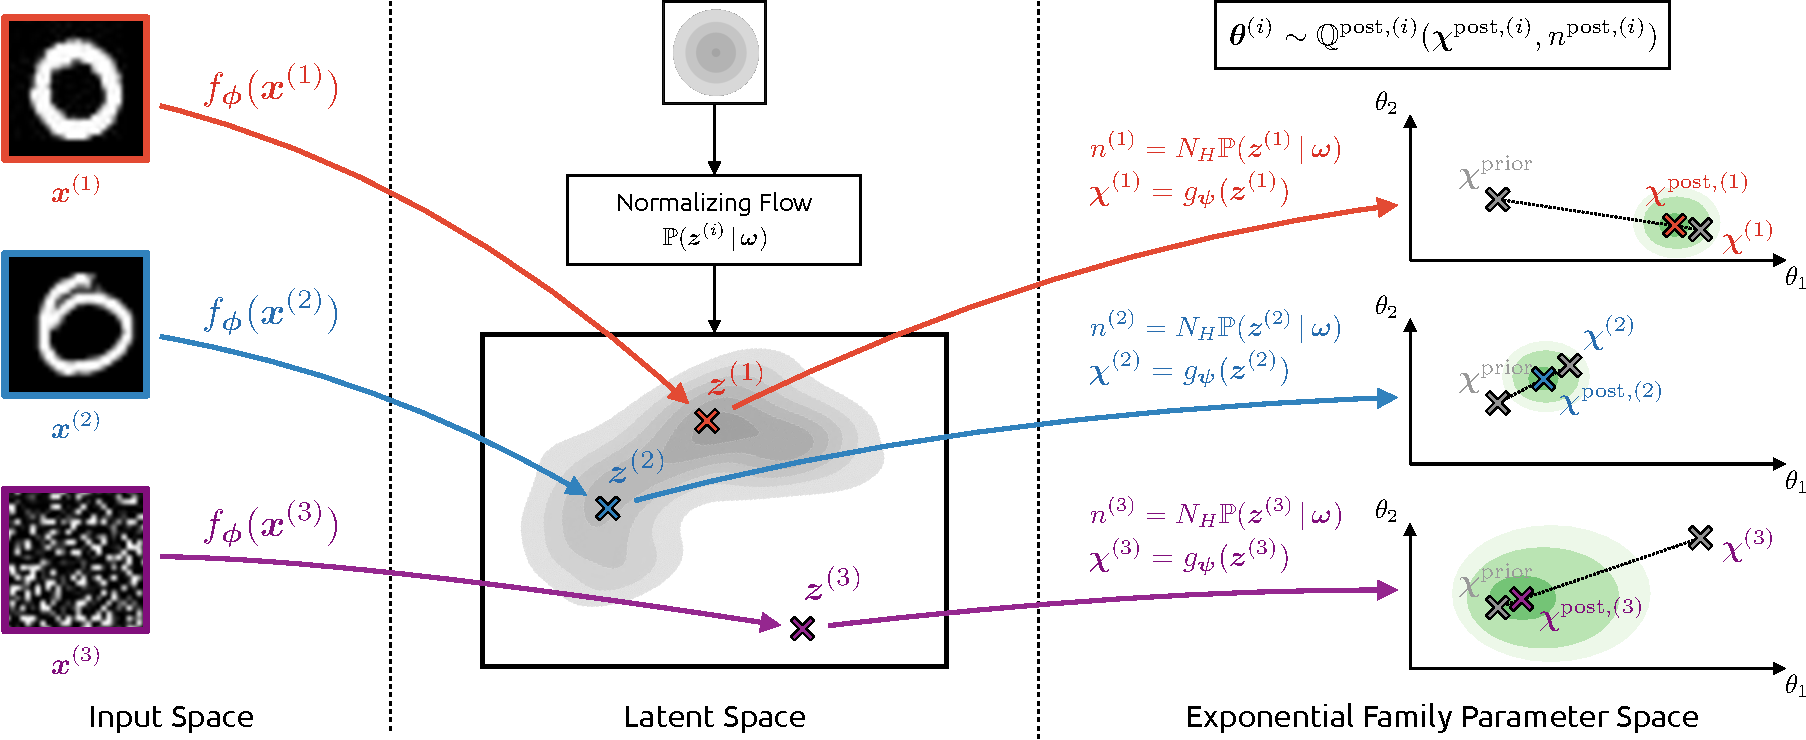
\includegraphics[width=.75\linewidth]{sections/007_iclr2022/resources/npn-crop.pdf}
    \caption{Overview of \NatPN{}. Inputs $\bm{x}^{(i)}$ are first mapped to a low-dimensional latent representation $\bm{z}^{(i)}$ by the encoder $f_{\bm{\phi}}$. From $\bm{z}^{(i)}$, the decoder $g_{\bm{\psi}}$ derives the parameter update $\bm{\chi}^{(i)}$ while a normalizing flow $\mathbb{P}_{\bm{\omega}}$ yields the evidence update $n^{(i)}$. Posterior parameters are obtained from a weighted combination of prior and update parameters according to $n^{\text{post},(i)}$.}
    \label{fig:npn}
    \vspace{-6mm}
\end{figure*}

Hence, \NatPNacro{} proposes a generic way to perform the input-dependent Bayesian update $\priorparam\dataix$, $\evidence\dataix$ for \emph{any} exponential family distribution in three steps (see Fig.~\ref{fig:npn}): \textbf{(1)} An encoder $f_{\bm{\phi}}$ maps the input $\x\dataix$ onto a low-dimensional latent vector $\z\dataix = f_{\phi}(\x\dataix) \in \real^H$ representing useful features for the prediction task (see left Fig.\ref{fig:npn}). Note that the architecture of the encoder can be arbitrarily complex. Then, \textbf{(2)} the latent representation $\z\dataix$ is used in two different ways to predict the parameter update $\priorparam\dataix$ and the evidence update $\evidence\dataix$ (see center Fig.\ref{fig:npn}). On the one hand, a linear decoder $g_{\bm{\psi}}$ is trained to output the parameter update $\priorparam\dataix = g_{\bm{\psi}}(\z\dataix) \in \real^L$ accounting for the aleatoric uncertainty. On the other hand, a single normalized density is trained to output the evidence update $\evidence\dataix = N_H\prob(\z\dataix \condition \bm{\omega})$ accounting for the epistemic uncertainty. The intuition is that increasing the evidence on training data during training forces the evidence everywhere else (incl. far from training data) to decrease thanks to the density normalization constraint. The constant $N_H$ is a certainty budget distributed by the normalized density $\prob(\z\dataix \condition \bm{\omega})$ over the latent representations $\z\dataix$ i.e. $N_H = \int N_H \prob(\z\dataix \condition \bm{\omega}) d\z\dataix = \int \evidence\dataix d\z\dataix$. In practice, we observed that scaling the certainty budget w.r.t. the latent dimension $H$ helped the density to cover larger volumes in higher dimension (see app.). Finally, \textbf{(3)} \NatPNacro{} computes the posterior parameters $\priorparam^{\text{post}, (\idata)}$ and $\evidence^{\text{post}, (\idata)}$ which can be viewed respectively as the mean and concentration of the posterior distribution (see right Fig.\ref{fig:npn}). Note that the posterior parameter $\priorparam^{\text{post}, (\idata)}$ is a simple weighted average of the prior parameter $\priorparam^\text{prior}$ and the update parameter $\priorparam\dataix$ as shown by Eq.~\ref{eq:parameter-update}.

\NatPNacro{} extends PostNet \citep{postnet} which also performs an input-dependent Bayesian update with density estimation. Yet, it has three crucial differences which lead to major practical improvements. First, the new exponential family framework is significantly more flexible and is not restricted to classification. Second, the Dirichlet $\bm{\alpha}$ parameter computation is different: \NatPNacro{} computes the $\priorparam$ parameters -- which can be viewed as standard softmax output -- and the $\evidence$ evidence separately (i.e. $\bm{\alpha} = \evidence \priorparam$) while PostNet computes one evidence pseudo-count per class. Third, \NatPNacro{} is computationally more efficient. It requires a single density while PostNet requires $\nclass$ densities.

\subsection{ID and OOD Uncertainty Estimates}
%\textbf{ID and OOD Uncertainty Estimates.} 
\NatPNacro{} intuitively leads to reasonable uncertainty estimation for the two limit cases of strong in-distribution (ID) and out-of-distribution (OOD) inputs (see red and purple samples in Fig.~\ref{fig:npn}). For very likely \emph{in-distribution} data (i.e. $\prob(\z\dataix \condition \bm{\omega}) \rightarrow \infty$), the posterior parameter overrules the prior (i.e. $\priorparam^{\text{post}, (\idata)} \rightarrow \priorparam\dataix$). Conversely, for very unlikely \emph{out-of-distribution} data (i.e. $\prob(\z\dataix \condition \bm{\omega}) \rightarrow 0$), the prior parameter takes over in the posterior update (i.e. $\priorparam^{\text{post}, (\idata)} \rightarrow \priorparam^\text{prior}$). Hence, the choice of the prior parameter should reflect the default prediction when the model lacks knowledge. We formally show under mild assumptions on the encoder that \NatPNacro{} predicts very low additional evidence ($\evidence\dataix \approx 0$) for (almost) any input $\x\dataix$ far away from the training data (i.e. $||\x\dataix|| \rightarrow + \infty$), thus recovering prior predictions (i.e. $\priorparam^{\text{post}, (\idata)} \approx \priorparam^\text{prior}$) (see proof in app.).
\begin{theorem}
\label{thm:oodom-guarantee}
Let a \NatPNacro{} model be parametrized with a (deep) encoder $f_{\phi}$ with ReLU activations, a decoder $g_{\psi}$ and the density $\prob(\z \condition \bm{\omega})$. Let $f_{\phi}(\x)= V^{(l)}\x + a^{(l)}$ be the piecewise affine representation of the ReLU network $f_{\phi}$ on the finite number of affine regions $Q^{(l)}$ \citep{understanding-nn-relu}. Suppose that $V^{(l)}$ have independent rows and the density function $\prob(\z \condition \bm{\omega})$ has bounded derivatives, then for almost any $\x$ we have \smash{$\prob(f_{\phi}(\delta \cdot \x) \condition \bm{\omega}) \underset{\delta \rightarrow \infty}{\rightarrow} 0$}. i.e the evidence becomes small far from training data.
\end{theorem}
This theorem only requires that the density avoids very unlikely pathological behavior with unbounded derivatives \citep{limit-existence-infinity}. A slightly weaker conclusion holds using the notion of limit in density if the density function does not have bounded derivatives \citep{integrable-infinity}. Finally, the independent rows condition is realistic for trained networks with no constant output \citep{overconfident-relu}. It advantageously leads \NatPNacro{} to consistent uncertainty estimation contrary to standard ReLU networks which are overconfident far from training data \citep{overconfident-relu}.

\subsection{Bayesian \NatPNacro{} Ensemble} 
%\textbf{Bayesian \NatPNacro{} Ensemble.} 
Interestingly, it is natural to extend the Bayesian treatment of a single \NatPNacro{} to an ensemble of \NatPNacro{} models (NatPE). An ensemble of $m$ \NatPNacro{} models is intuitively equivalent to performing $m$ successive Bayesian updates using each \NatPNacro{} member separately. More formally, given an input $\x\dataix$ and an ensemble of $m$ jointly trained \NatPNacro{} models, the Bayesian update for the posterior distribution becomes ${\priorparam^{\text{post}, (\idata)} = \frac{\evidence^\text{prior}\priorparam^\text{prior} + \sum_k^{m} \evidence_k\dataix \priorparam_k\dataix}{\evidence^\text{prior} + \sum_k^{m} \evidence_k\dataix}}$ and ${\evidence^{\text{post}, (\idata)} = \evidence^\text{prior} + \sum_k^{m} \evidence_k\dataix}$. %which is equivalent to having observed $m$ sets of \smash{$\evidence_k\dataix$} pseudo observations. %$\{\y_k^{(j)}\}_{j}\dataix$ such that $\sum_{j}^{\evidence_m\dataix} \y^{(j)} = \priorparam_k\dataix$. 
Note that the standard Bayesian averaging which is used in many ensembling methods \citep{bayesian-ensemble-learning,ensembles,batch-ensembles,hyper-ensembles} is different from this Bayesian combination. While Bayesian averaging assume that only one model is correct, the Bayesian combination of \NatPNacro{} allows \emph{more} or \emph{none} of the models to be ``expert'' for some input  \citep{bayesian-averaging-to-combination}. For example, an input $\x\dataix$ unfamiliar to every model $m$ (i.e. $\evidence_m\dataix \approx 0$) would recover the prior default prediction $\priorparam^\text{prior}, \evidence^\text{prior}$. Existing models already had similar properties for Bayesian combination of classifiers \citep{bayesian-classifier-combination, dynamic-bayesian-combination-classifiers}.

\subsection{Optimization}
\label{sec:optimization}

The choice of the optimization procedure is of primary importance in order to obtain both high-quality target predictions and uncertainty estimates regardless of the task.

\textbf{Bayesian Loss.} We follow \citet{postnet} and aim at minimizing the Bayesian formulation:
%
\begin{equation}\label{eq:bayesian-loss}
    \mathcal{L}\dataix = - \underbrace{\expectation_{\expparam\dataix \sim \prior^{\text{post},(\idata)}}[\log \prob(\y\dataix\condition \expparam \dataix)]}_\text{(i)} - \underbrace{\entropy[\prior^{\text{post},(\idata)}]}_\text{(ii)}
\end{equation}
%
where $\entropy[\prior^{\text{post},(\idata)}]$ denotes the entropy of the predicted posterior distribution $\prior^{\text{post},(\idata)}$. Similarly to the ELBO loss, this loss is guaranteed to be optimal when the predicted posterior distribution is close to the true posterior distribution $\prior^*(\expparam \condition \x\dataix)$ i.e. $\prior^{\text{post},(\idata)} \approx \prior^*(\expparam \condition \x\dataix)$ \citep{update-belief-propagation, PAC-bayesian_estimator, opt-info-processing_bayes}. However, this loss is generally \emph{not} equal to the ELBO loss especially for real valued targets i.e. $y \in \real$ (see app.). The term \textbf{(i)} is the expected likelihood under the predicted posterior distribution. It can be viewed as the Uncertain Cross Entropy (UCE) loss \citep{uceloss} which is known to reduce uncertainty on observed data. The term \textbf{(ii)} is an entropy regularizer acting as a prior which favors uninformative distributions $\prior^{\text{post},(\idata)}$ with high entropy. In our case, we assume the likelihood $\prob(\y\dataix\condition\expparam\dataix)$ and the posterior $\prior^{\text{post},(\idata)}$ to be members of the exponential family. We take advantage of the convenient computations for such distributions and derive a more explicit formula for the Bayesian formulation \eqref{eq:bayesian-loss} (see derivation in the appendix):
%
\begin{equation}\label{eq:nll-entropy}
    \begin{aligned}
    \mathcal{L}_\lambda\dataix &\propto \expectation[\expparam]^T \bm{u}(y\dataix) - \expectation[A(\bm{\expparam})] - \lambda\entropy[\prior^{\text{post},(\idata)}]
    \end{aligned}
\end{equation}
%
where $\lambda$ is an additional regularization weight tuned with a grid search. Note that the term $\expectation[\expparam]^T \bm{u}(y\dataix) $ favors a good alignment of the expected sufficient statistic $\expectation[\expparam] = \priorparam$ with the observed sufficient statistic $\bm{u}(y\dataix)$. In practice, all terms can be computed efficiently in closed form for most exponential family distributions (see examples in Tab.~\ref{tab:summary_exp_dist}). In particular, simplifications are possible when the conjugate prior distribution is also in an exponential family which is often the case. Ultimately Eq.~\eqref{eq:nll-entropy} applies to \emph{any} exponential family distribution unlike \citet{postnet}.

\textbf{Optimization Scheme.} \NatPNacro{} is fully differentiable using the closed-form Bayesian loss. Thus, we train the encoder $f_{\bm{\phi}}$, the parameter decoder $g_{\bm{\psi}}$ and the normalizing flow $\prob(\z\dataix \condition \bm{\omega})$ w.r.t. parameters $\bm{\phi}, \bm{\psi}, \bm{\omega}$ jointly. Further, we observed that ``warm-up training'' \citep{warm-start} and ``fine-tuning'' \citep{fine-tuning-continuous} of the density helped to improve uncertainty estimation for more complex flows and datasets. Thus, we train the normalizing flow density to maximize the likelihood of the latent representations before and after the joint optimization while keeping all other parameters fixed.

\subsection{Model Limitations} \label{sec:limitations}

\textbf{Task-Specific OOD.} Previous works show that density estimation is unsuitable for acting on the raw image input \citep{anomaly-detection,deep-generative,typicality_OOD_generative} or on a non-carefully transformed space \citep{perfect-density-no-ood-guarantee}. To circumvent this issue, \NatPNacro{} does not perform OOD detection directly on the input but rather fits a normalizing flow on a learned space. In particular, the latent space is \textbf{(1)} low-dimensional, \textbf{(2)} task-specific and \textbf{(3)} encodes meaningful semantic features. Similarly, \citet{postnet, why-nf-fail-ood, density-states-ood, contrastive-ood} already improved OOD detection of density-based methods by leveraging a task-induced bias or low-dimensional statistics. In the case of \NatPNacro{}, the low-dimensional latent space has to contain relevant features to linearly predict the sufficient statistics required for the task. For example, \NatPNacro{} aims at a linearly separable latent space for classification. The downside is that \NatPNacro{} is capable of detecting OOD samples only with respect to the considered task and requires labeled examples during training. As an example, \NatPNacro{} likely fails to detect a change of image color if the task aims at classifying object shapes and the latent space has no notion of color. Hence, we underline that \NatPNacro{} comes with a task-dependent OOD definition, which is a reasonable choice in practice.

\textbf{Model-Task Mismatch.} Second, we emphasize that the uncertainty estimation quality of \NatPNacro{} for (close to) ID data depends on the convergence of the model, the encoder architecture (e.g. MLP, Conv., DenseDepth \citep{dense-depth}) and the target distribution (e.g. Poisson, Normal distributions) choice which should match the task needs. However, we show \emph{empirically} that \NatPNacro{} provides high quality uncertainty estimates in practice on a wide range of tasks. Further, we show \emph{theoretically} that \NatPNacro{} leads to uncertain prediction far away from training data for \emph{any} exponential family target distributions. In comparison, \citet{provable-uncertainty} showed akin guarantees for classification only.